\documentclass[tikz,border=8pt]{standalone}
% Shared preamble for the bootqcc TikZ figures.
\usepackage[T1]{fontenc}
\usepackage{helvet}
\renewcommand{\familydefault}{\sfdefault}
\usepackage{amsmath}
\usetikzlibrary{arrows.meta,positioning,shapes.geometric,fit,backgrounds,calc}

\definecolor{navy}{HTML}{1F3A5F}
\definecolor{sky}{HTML}{5AA9E6}
\definecolor{coral}{HTML}{FF6B6B}
\definecolor{slate}{HTML}{6B7A8F}

\tikzset{
  box/.style={rectangle, rounded corners=4pt, draw=navy, fill=sky!15, thick,
              align=center, minimum height=1.0cm, inner sep=6pt, text width=4.6cm},
  inbox/.style={rectangle, rounded corners=4pt, draw=slate, fill=slate!10, thick,
              align=center, minimum height=0.9cm, inner sep=5pt, text width=3.0cm,
              font=\small},
  io/.style={trapezium, trapezium left angle=72, trapezium right angle=108,
             draw=navy, fill=white, thick, align=center, minimum height=1.2cm,
             inner sep=5pt, text width=3.0cm},
  result/.style={rectangle, rounded corners=8pt, draw=coral, fill=coral!10, thick,
              align=center, minimum height=1.0cm, inner sep=6pt, text width=4.0cm},
  term/.style={rectangle, rounded corners=12pt, draw=navy, fill=navy, text=white,
               thick, align=center, minimum height=0.9cm, inner sep=6pt, text width=4.2cm},
  dec/.style={diamond, aspect=2.6, draw=navy, fill=white, thick, align=center,
              inner sep=0pt, text width=2.7cm, font=\small},
  err/.style={rectangle, rounded corners=4pt, draw=coral, fill=coral!15, thick,
              align=center, minimum height=0.9cm, inner sep=6pt, text width=3.2cm},
  arr/.style={-{Latex[length=3mm]}, thick, navy},
  lab/.style={font=\footnotesize\bfseries, text=navy, fill=white, inner sep=1.5pt},
  phase/.style={rounded corners=8pt, draw=navy!45, dashed, thick, inner sep=12pt},
}

\begin{document}
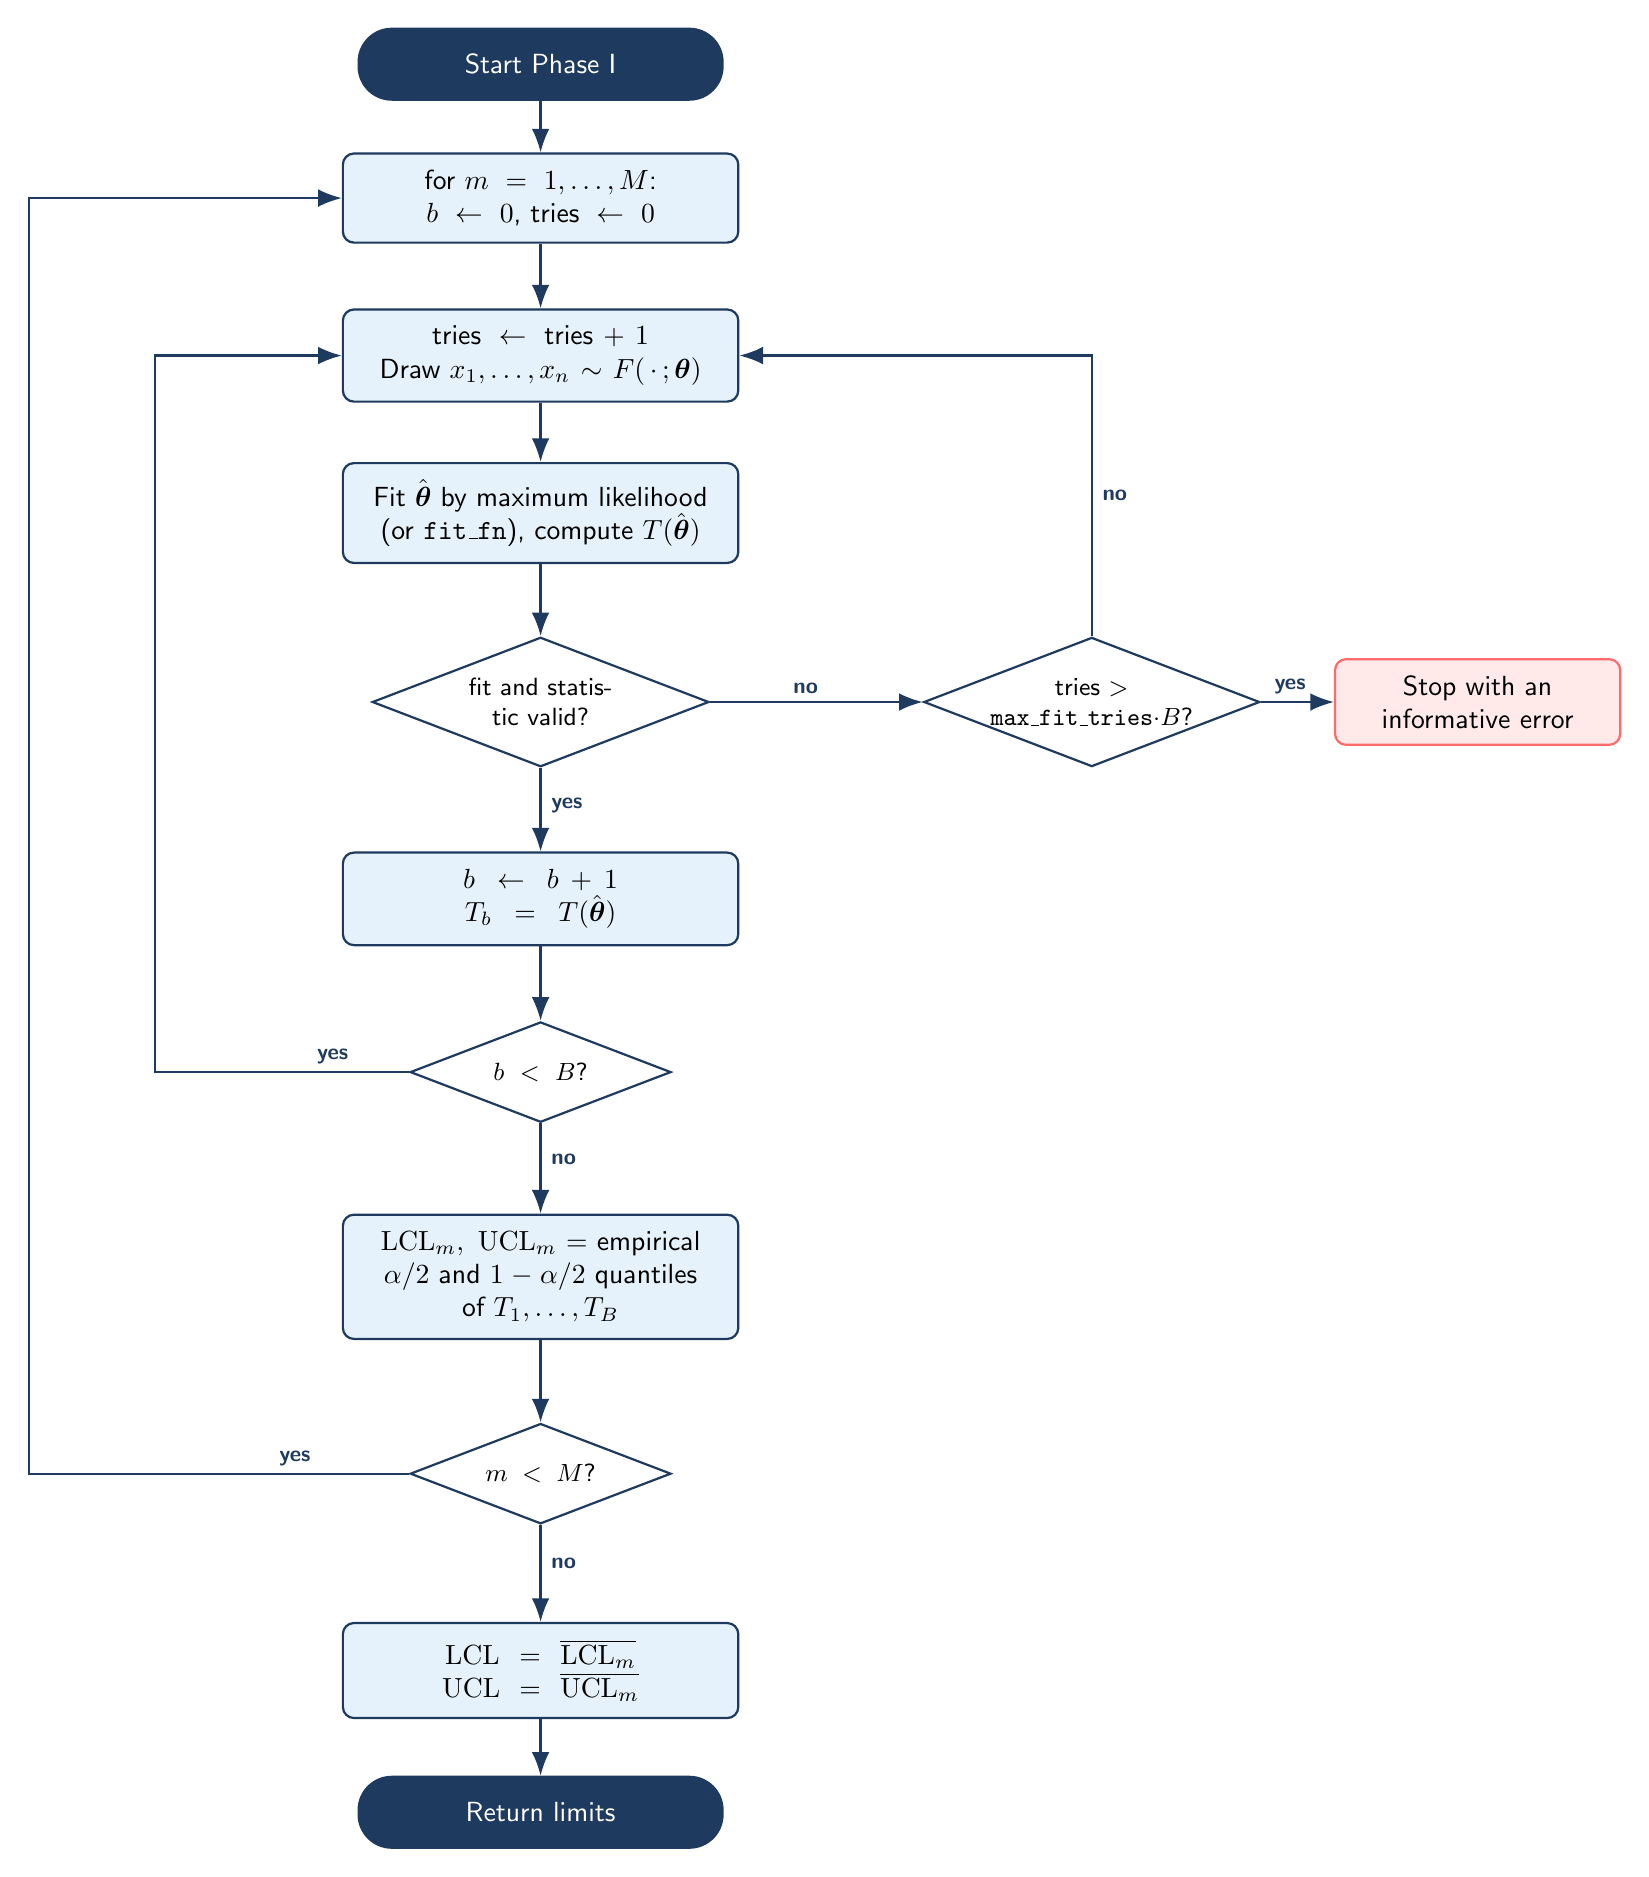
\begin{tikzpicture}

  \node[term] (start) at (0,0) {Start Phase I};
  \node[box]  (reset) at (0,-1.7)
    {for $m=1,\dots,M$:\\ $b\leftarrow 0$, $\text{tries}\leftarrow 0$};
  \node[box]  (draw)  at (0,-3.7)
    {$\text{tries}\leftarrow\text{tries}+1$\\ Draw $x_1,\dots,x_n\sim F(\,\cdot\,;\boldsymbol\theta)$};
  \node[box]  (fit)   at (0,-5.7)
    {Fit $\hat{\boldsymbol\theta}$ by maximum likelihood\\ (or \texttt{fit\_fn}), compute $T(\hat{\boldsymbol\theta})$};
  \node[dec]  (valid) at (0,-8.1) {fit and statistic valid?};
  \node[box]  (store) at (0,-10.6)
    {$b\leftarrow b+1$\\ $T_b = T(\hat{\boldsymbol\theta})$};
  \node[dec]  (bB)    at (0,-12.8) {$b<B$?};
  \node[box]  (quant) at (0,-15.4)
    {$\mathrm{LCL}_m,\ \mathrm{UCL}_m$ = empirical\\ $\alpha/2$ and $1-\alpha/2$ quantiles\\ of $T_1,\dots,T_B$};
  \node[dec]  (mM)    at (0,-17.9) {$m<M$?};
  \node[box]  (final) at (0,-20.4)
    {$\mathrm{LCL}=\overline{\mathrm{LCL}_m}$\\ $\mathrm{UCL}=\overline{\mathrm{UCL}_m}$};
  \node[term] (end)   at (0,-22.2) {Return limits};

  % failure branch
  \node[dec] (give)  at (7.0,-8.1) {tries $>$ \texttt{max\_fit\_tries}$\cdot B$?};
  \node[err] (error) at (11.9,-8.1) {Stop with an informative error};

  % main flow
  \draw[arr] (start) -- (reset);
  \draw[arr] (reset) -- (draw);
  \draw[arr] (draw)  -- (fit);
  \draw[arr] (fit)   -- (valid);
  \draw[arr] (valid) -- node[lab, pos=0.45, right=2pt] {yes} (store);
  \draw[arr] (store) -- (bB);
  \draw[arr] (bB)    -- node[lab, pos=0.4, right=2pt] {no} (quant);
  \draw[arr] (quant) -- (mM);
  \draw[arr] (mM)    -- node[lab, pos=0.4, right=2pt] {no} (final);
  \draw[arr] (final) -- (end);

  % failed fit: give up when the try budget is used up, otherwise redraw
  \draw[arr] (valid) -- node[lab, pos=0.45, above=1pt] {no} (give);
  \draw[arr] (give)  -- node[lab, pos=0.4, above=1pt] {yes} (error);
  \draw[arr] (give.north) |- node[lab, pos=0.25, right=2pt] {no} (draw.east);

  % inner loop over b
  \draw[arr] (bB.west) -- node[lab, pos=0.3, above=1pt] {yes} (-4.9,-12.8) |- (draw.west);
  % outer loop over m
  \draw[arr] (mM.west) -- node[lab, pos=0.3, above=1pt] {yes} (-6.5,-17.9) |- (reset.west);
\end{tikzpicture}
\end{document}
